\chapter{Introduction}  \label{ch:intro}
\graphicspath{{introduction/figures/}}

\begin{flushright}
\textit{``More data usually beats better algorithms''}\\
 Anand Rajaraman

\end{flushright}

Business Intelligence (BI) has always been about creating new insight for business by converting data into meaning that can be shared between people to drive change in the organization. One key aspect of creating meaning is driving a common shared understanding of information also known as Semantics.

Classic BI and even the newer Agile Visualization tools focus much of their selling features on attractive and unique visualizations, but preparing data for those visualizations still remains the far more challenging task in most BI projects large and small. self-service data provisioning aims at tackling this problem by providing intuitive dataset discovery, acquisition and integration techniques intuitively to the end user.

\section{Context and Motivation} \label{sec:motivation}

Enterprises use a wide range of heterogeneous information systems in their business activities such as Enterprise Resource Planning (ERP), Customer Relationships Management (CRM) and Supply Chain Management (SCM) systems. An enterprise distributed IT landscape contains multiple systems using different technologies and data standards~\cite{Mihindukulasooriya:COLD:13}. In addition to this heterogeneity, the amount of information in enterprise databases and on-line data stores expands exponentially each year. Enterprise Big Data isn't big in volume only, but in the associated file formats. The information is also often stored often in unstructured and unknown formats.

Data integration is the problem of combining data residing at different sources, and providing the user with a unified view of these data~\cite{Lenzerini:SIGMOD:02}. In large enterprises, it is a time and resource costly task. Various approaches have been introduced to solve this integration challenge. These approaches were primarily based on XML as the data representation syntax, Web Services to provide the data exchange protocols and Service Oriented Architecture (SOA) as a holistic approach for distributed systems architecture and communication~\cite{Frischmuth:ISWC:13,Frischmuth:SemWebJorunal:12}. However, it was found that these technologies are no sufficient to solve the integration problems in large enterprises. Recently, ontology-based data integration approaches have been suggested where ontologies are used to describe the data, queries and mappings between them~\cite{Wache:IJCAI:01}. A slightly different approach is the use of the Linked Data paradigm~\cite{Bizer:IJSWIS:09} for integrating enterprise data. Enterprises like Google and Microsoft are not only using the Linked Data integration paradigm for their information systems, but are also aiming at building enterprise knowledge bases (like the Google Knowledge Graph powered in part by Freebase\footnote{\url{http://freebase.com}}) that will act as a crystallization point for their structured data.

Data becomes more useful when it is open, widely available, in shareable formats and when advanced computing and analysis can yield from it. The quality and amount of structured knowledge available on the web make it now feasible for companies to mine this huge amount of public data and integrate it in their next-generation enterprise information management systems. An example of this external data is the Linked Open Data (LOD) cloud. From 12 datasets cataloged in 2007, it has grown to nearly 1000 datasets containing more than 82 billion triples\footnote{\url{http://datahub.io/dataset?tags=lod}}~\cite{Bizer:IJSWIS:09}. Data is being published by both the public and private sectors and covers a diverse set of domains from life sciences to media or government data. The LOD cloud is potentially a gold mine for organizations and individuals who are trying to leverage external data sources in order to produce more informed business decisions~\cite{Boyd:Article:11}. This external data can be accessed through public data portals like \texttt{Datahub.io} and \texttt{publicdata.eu} or private ones like \texttt{quandl.com} and \texttt{enigma.io}. Analyzing this new type of data within the context of existing enterprise data should bring them new or more accurate business insights and allow better recognition of sales and market opportunities~\cite{LaValle:MIT:11}.

\section{Use Case Scenario}

To enable wide scale and efficient integration of data, there are some efforts needed from various sides. In this thesis, we tackle the issues and challenges from the point of views of two personae:

\begin{itemize}
\item \textbf{Data Analyst:} A Data Analyst is an experienced professional who is able to collect and acquire data from multiple data sources, filter and clean data, interpret and analyze results and provide ongoing reports.
\item \textbf{Data Portal Administrator:} A Data Portal Administrator monitors the overall health of the portal. He oversees the creation of users, organizations and datasets. Administrators try to ensure a certain data quality level by continuously checking for spam and manually enhancing dataset descriptions and annotations.
\end{itemize}

In our scenario, \textbf{Bob} is a Data Analyst working with the Ministry of Transport in France. His favorite tool for crunching, manipulating and visualizing data is SAP Lumira~\footnote{\url{http://saplumira.com/}}. Bob received a memo from the management to create a report comparing the number of car accidents that occurred in France for that year, to its counterpart in the United Kingdom (UK). In addition, he was asked to highlight accidents related to illegal consumption of Alcohol in both countries.

After examining the ministry's records, Bob was able to collect the data needed to create his report for the French side. Bob issued an official request to the Department of Transport in UK  to collect the data needed. However, Bob knows that the process takes long time and the management needs the report within days. Bob is familiar with the Open Data movement and starts his journey searching through different data portals in the UK.

\textbf{Mark} is a Data Portal Administrator for the \texttt{data.gov.uk}. He continuously oversees the processes of acquiring, preparing and publishing datasets. Mark tries always to ensure that the data published is of high quality and contains sufficient attached metadata to easily enable search an discovery. Mark often receives complaints about inaccurate or spam datasets. He manually removes and fix errors while keeping open communication channels with the data-publishing departments.

\section{Research Challenges} \label{sec:challenges}

In the scenario presented above, both publishers (Data Portal Administrators) and users (Data Analysts) need pragmatic solutions that help them in their tasks. To enable that, there are some challenging research questions that have to be addressed. These challenges are organized in three main types as the following:

\subsection{Dataset Integration and Enrichment}
\begin{itemize}
	\item The enterprise heterogeneous data sources raise tremendous challenges. They have inherently different file formats, access protocols or query languages. They possess their own data model with different ways of representing and storing the data. Data across these sources may be noisy (e.g. duplicate or inconsistent), uncertain or be semantically similar yet different~\cite{Avitha:EuroJorunal:11}. Integration and provision of a unified view for these heterogeneous and complex data structures therefore require powerful tools to map and organize the data.
	\item Attaching metadata and Semantic information to instances can be tricky. An entity is usually not associated with a single generic type in the knowledge base, but rather with a set of specific types which can be relevant or not given the context. The challenging task is finding the most relevant entity type within a given context.
	\item Entities play a key role in knowledge bases in general and in the Web of Data in particular. Entities are generally described with a lot of properties, this is the case for DBpedia. It is, however, difficult to assess which ones are more ``important'' than others for particular tasks such data augmentation and visualizing the key facts of an entity.
	\item Social Networks are not just gathering Internet users into groups of common interests, they are also helping people follow breaking news, contribute to online debates or learn from others. They are transforming Web usage in terms of users' initial entry point, search, browsing and purchasing behavior. Integrating information from these Social Networks can be tricky due to the vast amount of data available which makes hard to spot what is relevant in a timely manner.
\end{itemize}

\subsection{Dataset Maintenance \& Discovery}
\begin{itemize}
\item Even though popular datasets like DBPedia\footnote{\url{http://dbpedia.org}} and Freebase are well known and widely used, there are other hidden useful datasets not being used. Indeed these datasets may be useful for specialized domains, however without proper registry of topics, it is difficult for users to find them~\cite{Lalithsena:WI:13}.
\item The growing amount of data requires rich metadata in order to reach its full potential. This metadata enables dataset discovery, understanding, integration and maintenance. Despite the various models and vocabularies describing datasets metadata, the ability to have an overview of the dataset by inspecting its metadata can be limited.
\item Users, organizations and governments are empowered to publish datasets. However, detecting spam and maintaining high quality data requires continuous attention and increasing manual efforts from portal administrators.
\end{itemize}

\subsection{Dataset Quality Control:} Linked Data consists of structured information supported by models, ontologies and vocabularies and contains query endpoints and links. This makes data quality assurance a challenge. Despite the fact that Linked Open Data quality is a trending and highly demanded topic, very few efforts are currently trying to standardize, track and formalize frameworks to issue scores or certificates that will help data consumers in their integration tasks.

\section{Thesis Contributions} \label{sec:contribution}

In this thesis, we propose a framework (see Figure~\ref{fig:architecutre_diagram}) to enable self-service data provisioning for internal and external data sources. The framework contributes to the three main challenges describes above. In summary, the main
contributions of this work are as follows:

\begin{figure}[!ht]
  \centering
  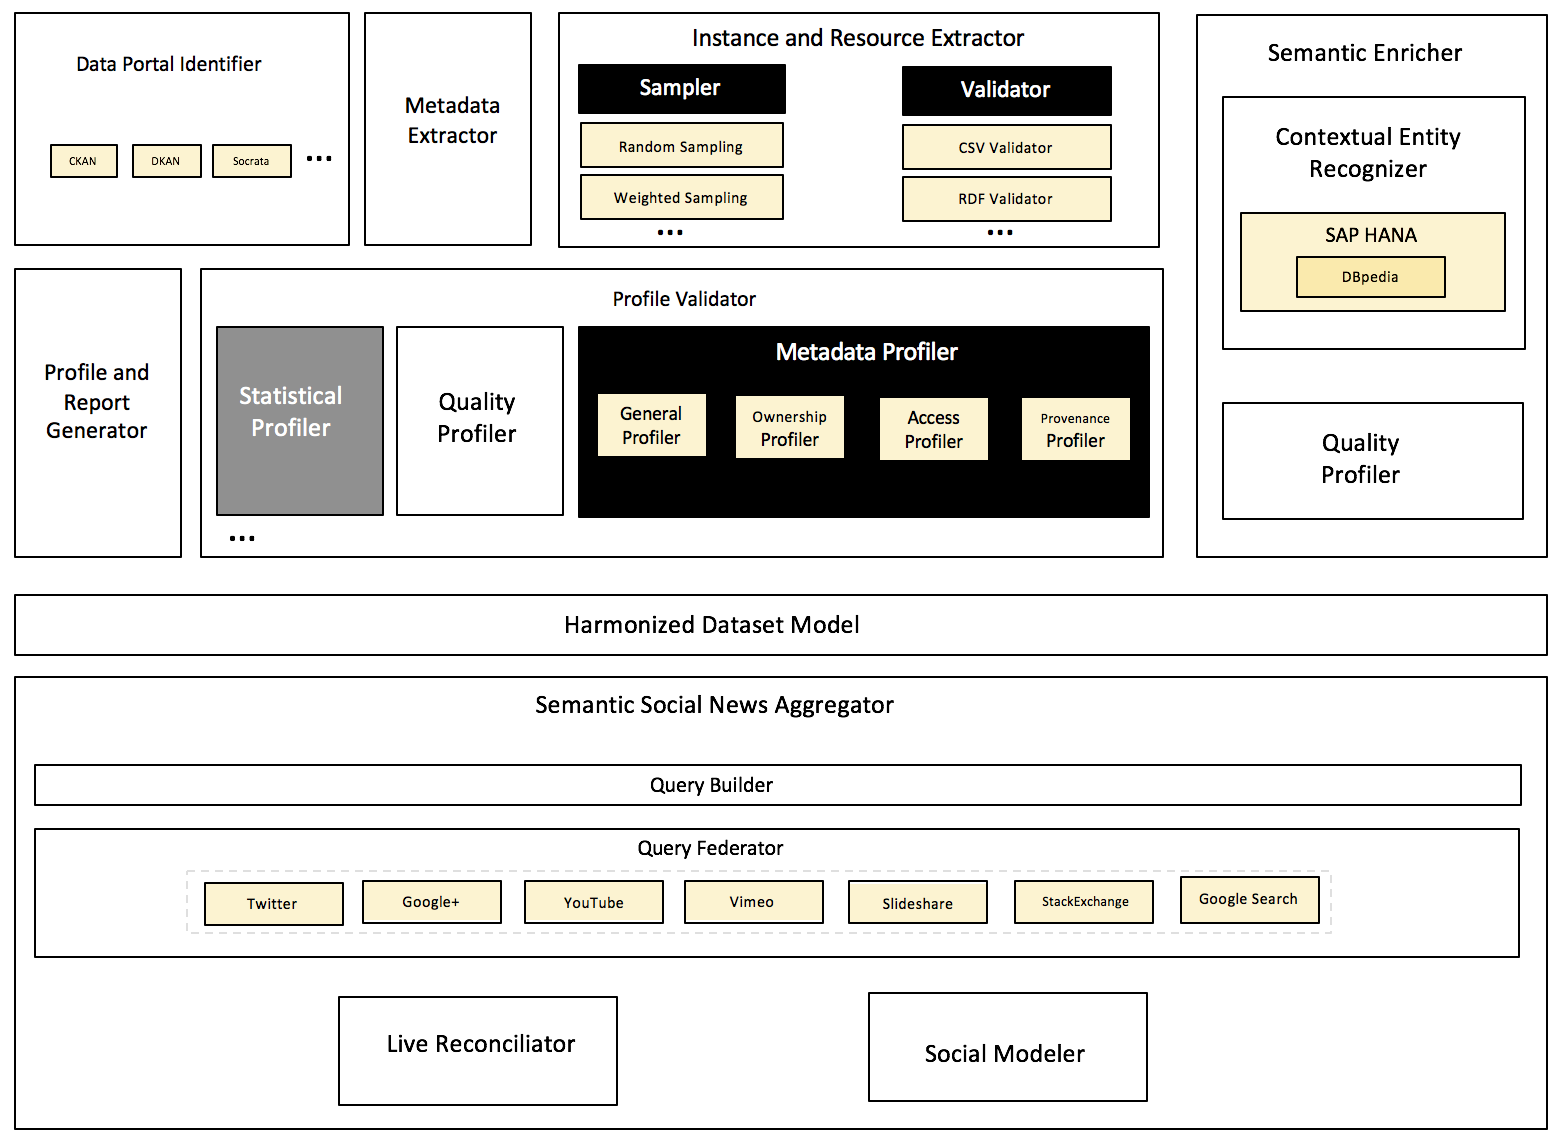
\includegraphics[scale=0.5]{architecutre_diagram.png}
  \caption{Processing pipeline for enabling self-service data provisioning}
  \label{fig:architecutre_diagram}
\end{figure}

\subsection{Contributions on Dataset Integration and Enrichment}
Regarding this aspect of our research, we have achieved the following tasks:
 \begin{itemize}
  \item We created a framework called RUBIX that enables mashing-up potentially noisy enterprise data and external data. The framework leverages reference knowledge bases to annotate data with a set of semantic concepts (metadata). One of the advantages of this metadata is to enhance the matching process of heterogeneous data sources \todo{add section}.
	\item The attached metadata by RUBIX can be further used to enrich existing datasets. However, concepts are often represented with a large set of properties. To better recommend the top ``important'' properties for a concept, we reversed engineer the choices made by Google when creating knowledge graph panels and compared them to preferences obtained from a user survey. We further represented these choices explicitly using the Fresnel vocabulary, so that any application could read this configuration file for deciding which properties of an entity is worth to enrich\todo{add section}.
	\item We have analyzed the landscape of dataset profiling tools and discovered gaps in the tools needed to create a profile that maps to the harmonized dataset model proposed. As a result, we propose a scalable automatic framework called Roomba for extracting, validating, correcting and generating descriptive linked dataset profiles. Roomba applies several techniques in order to check the validity of the metadata provided and to generate descriptive and statistical information for a particular dataset or for an entire data portal\todo{add section}.
	\item We presented the results of running Roomba over various data portals. We focused on analyzing the LOD cloud group hosted in the Datahuba and discovered that the general state of the examined datasets needs attention as most of them lack informative access information and their resources suffer low availability\todo{add section}.
	\item Aggregating relevant social news is not an easy task. We implemented an Application Programming Interface (API) that enables semantic social news aggregation called SNARC. we implemented a Google Chrome extension leveraging SNARC's capabilities to enable users to discover what is happening instantly and without the need to navigate away from the current page\todo{add section}.
\end{itemize}

\subsection{Contributions on Dataset Maintenance \& Discovery}

\begin{itemize}
	\item We surveyed the landscape of various models and vocabularies that described datasets on the web. Since establishing a common vocabulary or model is the key to communication, we identified the need for an harmonized dataset metadata model containing sufficient information so that consumers can easily understand and process datasets (Section~\ref{section:datasetModels}).
	\item We implemented a set of mappings between each properties of the surveyed models. This has lead to the design of HDL, a harmonized dataset model, that takes the best out of these models and extends them to ensure complete metadata coverage to enable data discovery, exploration and reuse(Section~\ref{section:hdl}).
\end{itemize}

\subsection{Contributions on Dataset Quality Control}
Concerning our contributions on Linked Data quality assessment, we have achieved the following tasks:
\begin{itemize}
	\item We proposed five principle classes to describe the quality of a particular linked dataset. For each class, we defined the principles that are involved at all stages of the data management process. We further refined these principles and propose a comprehensive objective quality framework applied to the Linked Open Data. We have built upon previous efforts with focus on objective data quality measures\todo{add section}.
	\item We notice that there is a plethora of tools (syntactic checkers or statistical profilers) that automatically check the quality of information at the entities level. Moreover, various tools can automatically check the models against the objective quality indicators mentioned. However, we notice a lack in automatic tools to check the dataset quality especially in its completeness, licensing and provenance measures. As a result, we extended Roomba to perform a set of data quality checks on Linked datasets.Our extension covers most of the quality indicators with its focus on completeness, correctness provenance and licensing\todo{add section}.
\end{itemize}

\section{Thesis Outline} \label{sec:outline}
The work presented in this thesis first describes a standard model to represent dataset profiles. Then it focuses on techniques to automatically generate and validate these profiles.

Chapter 2 is dedicated to overview the background of our work including the research in data integration and enrichment and some paradigms related to Semantic Web. We first introduce the basic concepts in the Semantic Web and the important aspects related to (Linked) Open Data. Then, we describe the various data integration techniques and the importance of external data to the enterprise.

The rest of this manuscript is composed of (N) major parts: